% File: solutions/ex6.tex

\begin{soluzione}{6}
    \begin{enumerate}
        \item \textbf{Spiegazione del fenomeno dell'aliasing}
        
        L'aliasing si verifica quando la frequenza di campionamento $f_s$ è inferiore al doppio della massima frequenza del segnale, $B$. Questa è una violazione della condizione del \textbf{Teorema di Nyquist}:
        \[
            f_s < 2B
        \]
        Nel nostro caso:
        \begin{itemize}
            \item Massima frequenza del segnale: $B = 100$ Hz.
            \item Frequenza di campionamento: $f_s = 150$ Hz.
        \end{itemize}
        Verifichiamo la condizione:
        \[
            150 \text{ Hz} < 2 \cdot 100 \text{ Hz} \implies 150 \text{ Hz} < 200 \text{ Hz}
        \]
        Poiché la condizione è vera, il campionamento introduce aliasing. In termini pratici, questo significa che quando lo spettro originale viene replicato a intervalli di $f_s$, le repliche sono troppo vicine e le loro "code" si sovrappongono. L'informazione delle alte frequenze della replica centrale si confonde (diventa indistinguibile) con quella delle basse frequenze delle repliche adiacenti.

        \item \textbf{Grafico dello spettro campionato con aliasing}

        Lo spettro campionato $\tilde{X}(f)$ è dato dalla somma delle repliche dello spettro originale $X(f)$, scalate di un fattore $1/T = f_s = 150$. Ogni replica ha un'altezza di picco di $1 \cdot 150 = 150$.
        \begin{itemize}
            \item La replica centrale ($k=0$) è centrata a $0$ Hz e si estende da $-100$ Hz a $100$ Hz.
            \item La replica a destra ($k=1$) è centrata a $f_s = 150$ Hz e si estende da $150-100 = 50$ Hz a $150+100=250$ Hz.
            \item La replica a sinistra ($k=-1$) è centrata a $-f_s = -150$ Hz e si estende da $-250$ Hz a $-50$ Hz.
        \end{itemize}
        La sovrapposizione (aliasing) avviene negli intervalli $[-100, -50]$ Hz e $[50, 100]$ Hz.

        \begin{center}
        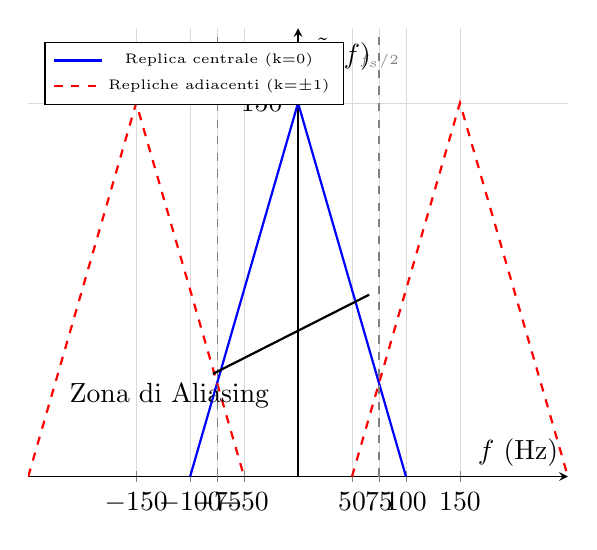
\begin{tikzpicture}
            \begin{axis}[
                axis lines=middle,
                xlabel=$f$ (Hz),
                ylabel=$\tilde{X}(f)$,
                xmin=-250, xmax=250,
                ymin=0, ymax=180,
                xtick={-150, -100, -75, -50, 0, 50, 75, 100, 150},
                ytick={150},
                grid=both,
                grid style={line width=.1pt, draw=gray!30},
                legend pos=north west,
                legend style={font=\tiny}
            ]
            
            % Replica centrale
            \addplot[blue, thick, domain=-100:100] {150 * (1 - abs(x)/100)};
            \addlegendentry{Replica centrale (k=0)}
            
            % Replica destra (aliasing)
            \addplot[red, thick, dashed, domain=50:250] {150 * (1 - abs(x-150)/100)};
            \addlegendentry{Repliche adiacenti (k=$\pm 1$)}

            % Replica sinistra (aliasing)
            \addplot[red, thick, dashed, domain=-250:-50] {150 * (1 - abs(x+150)/100)};

            % Linee guida per la banda di Nyquist
            \draw[dashed, gray] (axis cs:-75, 0) -- (axis cs:-75, 180);
            \node[above, gray, font=\tiny] at (axis cs:-75, 160) {$-f_s/2$};
            \draw[dashed, gray] (axis cs:75, 0) -- (axis cs:75, 180);
            \node[above, gray, font=\tiny] at (axis cs:75, 160) {$f_s/2$};

            % Indicazione dell'aliasing
            \node[pin={[pin edge={black, thick}, pin distance=1.5cm]220:{Zona di Aliasing}}] at (axis cs:75,75) {};

            \end{axis}
        \end{tikzpicture}
        \end{center}
        Il grafico mostra la replica centrale (blu) che si sovrappone con le code delle repliche adiacenti (rosse). All'interno della banda fondamentale (delimitata dalle linee grigie a $\pm f_s/2 = \pm 75$ Hz), lo spettro che verrebbe catturato da un filtro di ricostruzione non è più un semplice triangolo, ma una versione distorta a causa della somma delle componenti che si sovrappongono.

    \end{enumerate}
\end{soluzione}